\documentclass{beamer}
\documentclass[xetex,mathserif,serif]{beamer}
\title[Crisis] % (optional, only for long titles)
{Adaptive Mesh Refinement}
\subtitle{1D Hyperbolic Problems}
\author[Author, A] % (optional, for multiple authors)
{S. Sinha\inst{1} \and K. J. Roche\inst{1,2}}
\institute[Universities Here and There] % (optional)
{
  \inst{1}%
  Department of Applied Mathematics\\
  University of Washington
  \and
  \inst{2}%
  High Performance Computing\\
  Pacific Northwest National Laboratory
}
\date[KPT 2004] % (optional)
{Presentation to AM574, Prof. R. J. Leveque presiding}
\subject{Computer Science}

\begin{document}
\frame{\titlepage}
  
  %get references out of the way first 
  \begin{frame}[allowframebreaks]
  \frametitle<presentation>{Main References for this Talk}    
  \begin{thebibliography}{10}    
%  \beamertemplatebookbibitems
 % \bibitem{Autor1990}
  %  A.~Autor.
   % \newblock {\em Introduction to Giving Presentations}.
    %\newblock Klein-Verlag, 1990.
  \beamertemplatearticlebibitems
  \bibitem{Berger1998}
    M.~Berger and R.~Leveque 
    \newblock Adaptive Mesh Refinement Using Wave-Propagation Algorithms for Hyperbolic Systems
    \newblock {\em SIAM J. Numer. Anal.}, 35(6):2298--2316, 1998.
    %berger thesis
      \beamertemplatearticlebibitems
  \bibitem{Berger1982}
    M.~Berger
    \newblock Adaptive Mesh Refinement for Hyperbolic Partial Differential Equations
    \newblock {\em PhD Thesis}, Department of Computer Science, Stanford University, Stanford, CA 94305, 1982.
  \end{thebibliography}
\end{frame}

%outline
  \begin{frame}
    \frametitle{Talk Outline}
    \begin{itemize}
    \item{Overview of Berger and Leveque AMR paper}
    \item{wave propagation formulation}
    \item{etc.}
    \end{itemize}
    %Content goes here
  \end{frame}
  
  \begin{frame}{Figure Example}
  The question is how does beamerclass place this ???
          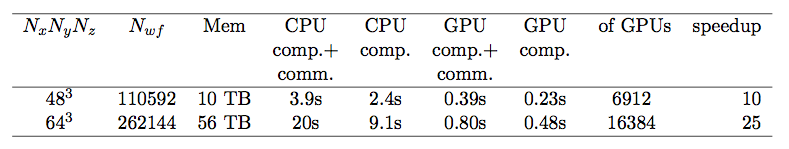
\includegraphics[height=2.5cm,width=10cm]{corrected-titan-4cmp-abm-cpu-gpu.png}
\end{frame}

  %frames with figures ... 
  \begin{frame}{Example of columns 1}
    \begin{columns}[c] % the "c" option specifies center vertical alignment
    \column{.5\textwidth} % column designated by a command
     Contents of the first column
    \column{.5\textwidth}
     Contents split \\ into two lines
    \end{columns}
\end{frame}
  
  %basic frame structure 
  \begin{frame}
    \frametitle{This is the second slide}
    \framesubtitle{A bit more information about this}
    %More content goes here
  \end{frame}
  \begin{frame}[fragile]

% for source code reference if needed -still not happy with this yet but we have time ... 
\frametitle{Source code}
 
\begin{lstlisting}[caption=First C example]
int main()
{
    printf("Hello World!");
    return 0;
}
\end{lstlisting}
\end{frame}
% etc
\end{document}